\documentclass[11pt]{article}

\usepackage[letterpaper,margin=0.75in]{geometry}
\usepackage{booktabs}
\usepackage{graphicx}
\usepackage{listings}
\usepackage{fixltx2e}
\usepackage{verbatim}
\usepackage{color}

\definecolor{dkgreen}{rgb}{0,0.6,0}
\definecolor{gray}{rgb}{0.5,0.5,0.5}
\definecolor{mauve}{rgb}{0.58,0,0.82}
\definecolor{orange}{RGB}{255,119,0}
\definecolor{purple2}{RGB}{153,0,153}

\setlength{\parindent}{1.4em}

\begin{document}

\lstset{
  language=Python,
  basicstyle=\small\ttfamily, % print whole listing small
  keywordstyle=\color{orange},
  keywordstyle={[2]\color{purple2}},
  identifierstyle=,           % nothing happens
  commentstyle=\color{dkgreen},% green comments
  stringstyle=\ttfamily\color{mauve},      % typewriter type for strings
  showstringspaces=false,     % no special string spaces
  numbers=left,
  numberstyle=\tiny\color{gray},
  numbersep=5pt,
  frame=tb,
}

\title{CS460 Lab 2 Report: Reliable Transport}

\author{Michael K. Eagar}

\date{February 23rd, 2014}

\maketitle

\section{Reliable Transport Implementation}

In order to implement the reliable transport protocol I started with Dr. Zappala's Stop and Wait implementation, and built upon it. In order to guarantee reliable transport I implemented a sliding window for sending packets. I removed the \textit{send()} method that was used to initialize the sending of packets, and replaced it with a \textit{load\_buffer} and a \textit{window\_init} method to load the data of the file being sent, and begin the sending process. I modified \textit{transfer.py} to call these methods instead of the send method from \textit{stopandwait.py}. My protocol is saved in the file \textit{my\_rtp.py}.\\

The Window initialization method calls the \textit{send\_if\_possible()} method, which has been modified to check if there are any open slots in the window to send additional packets, and sends one by calling \textit{send\_one\_packet()}. When a packet is sent the retransmit timer is set if it is not currently running. If the timer expires before the packet it's timing is ACKed, then that packet will be re-sent. Here is the \textit{window\_init()} method:

\lstinputlisting[breaklines = true, firstline = 68, lastline = 71, caption = window\_init()]{./my_rtp.py}
\vspace{0.25cm}

When the packet is received at it's destination node the sequence number is checked against the one the node is expecting. If the packet sequence is greater than or equal to the sequence the node is expecting, then the packet is added to the receive buffer and the buffer is sorted. If the first packet in the buffer is the one expected, then it is written to disk and the buffer is checked for subsequent packets until a missing one is detected. An ACK is then sent for the next packet that the receiving node expects.\\

When an ACK is received at the sending node it is passed to the \textit{handle\_packet()} method and it is checked to see if it is within the window range of packets sent out. If it is, the sending node calls \textit{slide\_window()} to slide the window forward to send more packets. In the \textit{slide\_window()} method the number of packets outstanding is decremented depending on the ACK number received. The window then slides forward so that its start is at the next packet after the ACK received. Additional packets can then be sent depending on slots available in the window. The process of sending packets, receiving ACKS and moving the window forward repeats until the entire file has been received at the destination node. Here are the \textit{handle\_packet()} method and the \textit{slide\_window()} method:

\lstinputlisting[breaklines = true, firstline = 28, lastline = 61, caption = handle\_packet()]{./my_rtp.py}
\vspace{0.25cm}

\lstinputlisting[breaklines = true, firstline = 71, lastline = 81, caption = slide\_window()]{./my_rtp.py}
\vspace{0.25cm}

\section{Testing}

In order to test my reliable transport protocol implementation I used Dr. Zappala's \textit{transfer.py} file as the basis for setting up my tests. I changed transfer.py to accept additional command line parameters, \textit{Queue size} and \textit{Window size}. These parameters are used to set up the simulated network and the window size for the protocol. The links between the two nodes are set with a bandwidth of 10 Mbps, and a propagation delay of 10 ms.\\

I then wrote a python script to run the eight tests in two sets by passing different command line parameters to \textit{transfer.py}:
\begin{enumerate}
  \item Set 1 - Window size of 3000 bytes (3 packets), transfer \textit{test.txt}
  \begin{enumerate}
    \item Loss rate of 0\%
    \item Loss rate of 10\%
    \item Loss rate of 20\%
    \item Loss rate of 50\%
  \end{enumerate}
  \item Set 2 - Window size of 10000 bytes (10 packets), transfer \textit{internet-architecture.pdf}
  \begin{enumerate}
    \item Loss rate of 0\%
    \item Loss rate of 10\%
    \item Loss rate of 20\%
    \item Loss rate of 50\%
  \end{enumerate}
\end{enumerate}

\vspace{0.25cm}

The python script is \textit{run\_lab2\_testing.py}, and must be run in the \textbf{lab2} directory. I saved the output results from my tests in the file \textit{testing.txt} which is in the \textbf{lab2/data} directory.

My reliable transport protocol passed all of the tests, successfully transferring the specified file each time.
\vspace{0.25cm}

\section{Experiments}

In order to run the experiments as required in the lab specifications, I used the same network configuration as used in the testing section, but set the \textit{queue size} to be 0\%. I wrote a python script to run the experiments by once again passing command line arguments to \textit{transfer.py}, varying the window size at 1000, 2000, 5000, 10000, 15000, and 20000 bytes. These window sizes correspond with 1, 2, 5, 10, 15, and 20 packets respectively. The script is \textit{run\_lab2\_experiments.py} and must be run in the \textbf{lab2} directory. The resulting output from the experiments is in the file \textit{experiments} in the \textbf{lab2/data} directory.
\vspace{0.25cm}

Figure 1 shows the average queuing delay per packet as window size is increased.  It shows that as window size increases, so does the average queuing delay. It seems to follow an exponential curve, but more data would be required in order to verify this.
\vspace{0.25cm}

\textit{Figure 1 - Average Queuing Delay vs Window Size}
\\
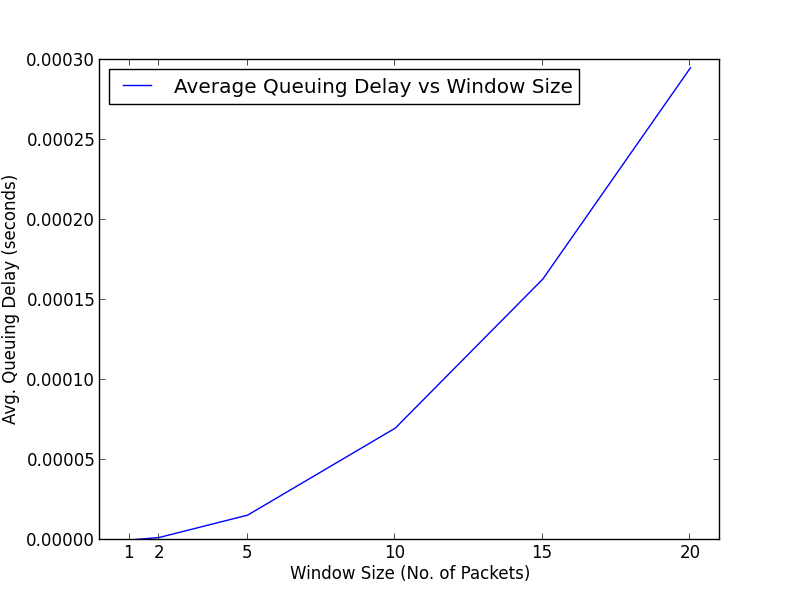
\includegraphics[width=13cm]{data/AvgQueuingDelayLinePlot}
\vspace{0.25cm}

Figure 2 below shows the throughput of the link as the window size increases. For the window sizes used in the experiment, throughput increases at a linear rate. This was interesting to me, as I had expected the throughput to cap off. It could be that larger window sizes would need to be tested in order to see the that in the results.
\\\\

\textit{Figure 2 - Throughput vs Window Size}
\\
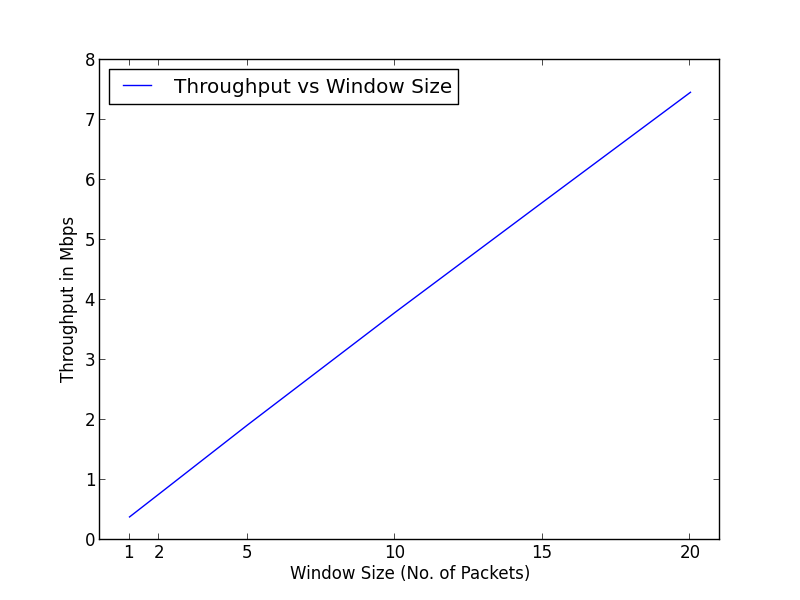
\includegraphics[width=13cm]{data/ThroughputLinePlot}

\end{document}
